\chapter{Grundlagen}

Das Grundlagenkapitel gibt eine Einführung und Übersicht über die verwendeten Begriffe und Konzepte, die im Weiteren dieser Arbeit von Bedeutung sind. Zunächst wird die Darstellung von Bildern behandelt und anschließend die Erhebung von charakteristischen Merkmalen aus Bildern, den Features. Hier genutzte Verfahren zur Detektion und Extraktion solcher Features werden im folgenden erläutert.\newline
In den folgenden Kapiteln wird ein Modell konzipiert und realisiert, dass eine Gruppierung von Bildern durch einen Autoencoder und Bag of Visual Words ermöglicht. Diese Verfahren werden tiefer in der Analyse betrachtet, hier soll jedoch der mathematische Hintergrund betrachtet werden. Aus diesem Grund wird, für den Bag of Visual Words, die Familie der k-means Algorithmen eingeführt. Da es sich bei einem Autoencoder um ein spezielles neuronales Netzwerk handelt, werden in diesem Kapitel  die Grundlagen neuronaler Netze vorgestellt.\newline
Im letzten Teil wird auf die Berechnung allgemein mathematischer Probleme auf Grafikkarten, dass GPU Computing, eingegangen. Durch den Einsatz von Grafikkarten können Berechnungen gerade bei großen Datenmengen stark beschleunigt werden, da diese massiv parallel auf den Daten arbeiten. Mit Nvidias CUDA wird ein Ausführungsmodell eingeführt, mit der sich Modelle wie der Bag of Visual Words und Autoencoder auf Nvidia Grafikkarten ausführen lassen.

\section{Bilder und Features}

Zunächst wird definiert wie ein Bild mathematisch aufgefasst wird, um eine effiziente Verarbeitung zu ermöglichen. Jedes Verfahren erwartet ein Bild als Eingabe. Verändern Algorithmen ein Bild, so geben sie die bearbeite Version wieder aus. Bei Analysen hingegen wird ein Bild nicht verändert, es wird auf Muster untersucht und die gefundenen Eigenschaften zurückgegeben. Diese Eigenschaften werden Features genannt. Der Prozess der Featuregewinnung ist in Detektion und Extraktion unterteilt und wird im Anschluss behandelt.

\subsection{Bilder}

Bei einem digitalen Bild handelt es sich um eine Matrix $I(x, y)$, welche Intensitätswerte enthält. Die Anzahl der Spalten $m$ und Zeilen $n$ entspricht dabei den Dimensionen des Bildes in Pixeln. Hier bezeichnen $(x, y)$ Indizes der Matrix und somit die einzelnen Pixel des Bildes. Die Darstellung in Matrixform eignet sich  sehr gut für Transformationen und Analysen des Bildes. Solche Verfahren betrachten oft jeden Pixel und oft eine Nachbarschaft dessen. Bei einer Nachbarschaft handelt es sich um die umliegenden Pixel zu einem ausgewählten Pixel. Die Größe der Nachbarschaft ist abhängig von dem Analyseverfahren: Beispielsweise umfasst die kleinstmögliche Nachbarschaft eines Pixels nur die direkt angrenzenden Pixel und ist somit eine $3 \times 3$ Matrix (mit dem Pixel als Zentrum). Formal werden diese Matrizen wie folgt dargestellt, wobei $n$ und $m$ wieder der Anzahl der Zeilen bzw. Spalten entsprechen:

$$
I(x, y) = \begin{bmatrix}
i_{0, 0}   & i_{0, 1}	& \dots	 & i_{0, n-1}   \\
i_{1, 0}   & i_{1, 1}   & \dots  & i_{1, n-1}   \\
\vdots	   & \vdots 	& \ddots & \vdots       \\
i_{m-1, 0} & i_{m-1, 1} & \dots	 & i_{m-1, n-1}
\end{bmatrix}
$$ 

Abhängig vom Typ des Bildes, besitzen die Pixel eine andere Struktur. In der Bilderverarbeitung und im Weiteren dieser Arbeit werden meist folgenden Arten von Bildern verwendet:
\begin{itemize}
	\item \textbf{Monochromatische Bilder} Diese Bilder werden nur in Graustufe dargestellt, daher besitzt ein Pixel genau einen Intensitätswert.
	\item \textbf{Multispektrale Bilder} Jeder Pixel besitzt einen Vektor an Werten. Im Falle eines Farbbildes enthält der Vektor drei Intensitätswerte für rot, grün und blau.
\end{itemize}
Die Intensität eines Pixels bzw. die Intensität seiner Vektoren wird mit in den meisten Programmen mit acht Bit dargestellt und umfasst daher 256 mögliche Werte. Dies ist für die meisten Anwendungen ausreichend und praktisch, da acht Bit genau einem Byte entsprechen und dies eine einfache computergestützt Darstellung und Verarbeitung ermöglicht. Die Werte für die Intensität werden im Folgenden normalisiert als Gleitkommazahlen im Intervall $[0, 1]$ verwendet, um unabhängig von dem Datentyp zu sein. 

\subsection{Feature Detektion und Extraktion}

Um Bilder zu vergleichen werden charakteristische Merkmale dieser betrachtet, die sogenannten Features. Ein Feature ist ein allgemeiner Begriff und enthält je nach Verfahren unterschiedliche Informationen. Dies ist notwendig, da nicht nur die Position oder Intensität eines Pixels, sondern auch generelle Eigenschaften von Interesse sind. Globale Verfahren berücksichtigen bei der Bewertung jeden Pixel des Bildes gleichermaßen, lokale hingegen betrachten nur ein kleine Fenster des Bildes, also einen Pixel und seine Nachbarschaft. Die Suche nach globalen Merkmalen, die ein Bild charakterisieren, kann aber keine Objekte und Details im Bild berücksichtigen. Hierfür eignet sich die Extraktion von lokalen Features. Um Objekte aus unterschiedlichen Perspektiven und in verschiedenen Größen wieder zu erkennen, ist es notwendig, dass die Features affin invariant sind. Abbildung \ref{img:liberty} zeigt dasselbe Objekt, jedoch rotiert, skaliert und verschoben. Ein Algorithmus sollte mit hoher Wahrscheinlichkeit erkennen, dass es sich hier um dasselbe Objekt handelt \cite{ifd2016}.

\begin{figure}
	\centering
	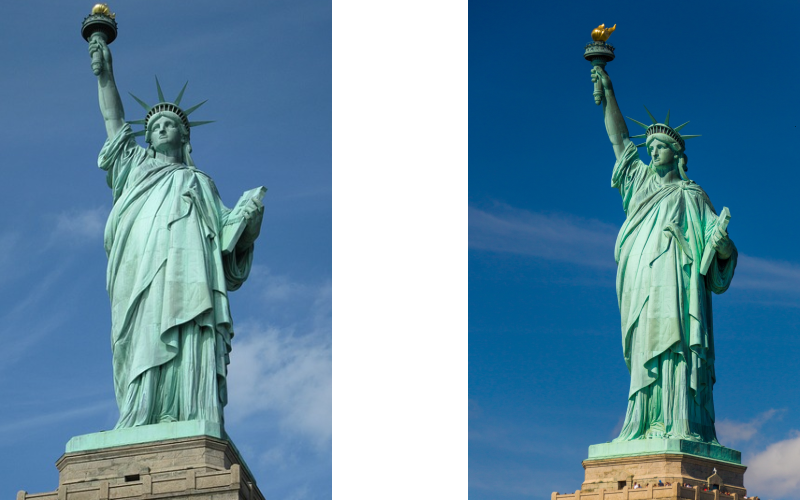
\includegraphics[scale=0.6]{images/liberty.png}
	\caption{Zwei Bilder mit dem gleichen Objekt aus unterschiedlicher Perspektive und in verschiedenen Lichtverhältnissen.}
	\label{img:liberty}
\end{figure}

Die Gewinnung der Features ist in die Schritte Detektion und Extraktion aufgeteilt: 

\begin{itemize}
	\item \textbf{Detektion} Ein Feature-Detektor in der Bildverarbeitung untersucht das Bild auf \glqq interessante \grqq  Regionen. Die Definition hängt hier maßgeblich vom verwendeten Verfahren ab. Allgemein wird zwischen Detektoren unterschieden die Ecken, Kanten und Regionen (BLOB) betrachten. Einige der Detektoren berücksichtigen hier auch mehr als eine Kategorie: Das Difference of Gaussians Verfahren dient beispielsweise der Erkennung von Ecken und Regionen. Als Ergebnis liefert ein Detektor eine Menge von Pixel und ggf. ihrer Nachbarschaften. Diese Pixel sind die sogenannten \textit{keypoints} und beschreiben, mit ihren Nachbarschaften, die eingangs erwähnten \glqq interessanten \grqq Stellen.\newline
	 Um praktisch einsetzbar zu sein, muss ein Detektor ein Feature, dass in verschiedenen Bildern auftaucht, zuverlässig erkennen. Hier sollte aber die angestrebte Allgemeinheit berücksichtigt werden: Ein Feature Detektor für medizinische Bilder, z.B. Röntgenaufnahmen, kann speziellere Annahmen treffen, als einer für eine allgemeine Bildsuche. In Abbildung \ref{img:keypoints} sind die durch einen SIFT-Detektor gefundenen \textit{keypoints} Farblich hervorgehoben.
	\item \textbf{Extraktion} Die Feature Extraktion erzeugt aus den vom Detektor gefundenen \textit{keypoints} und seinen lokalen Informationen den Deskriptor. Ein Feature-Deskriptor ist eine kompakte Darstellung eines Features. Die \textit{keypoints} und deren Nachbarschaften werden in Zahlen kodiert. Diese Sequenz wird als ein Vektor notiert, sodass auch von Feature-Vektor gesprochen wird. Einige Verfahren reichen den Deskriptor mit zusätzlichen Informationen an, z.B. über die Stärke eines Gradienten bei der Kantendetektion.
\end{itemize}

\begin{figure}
	\centering
	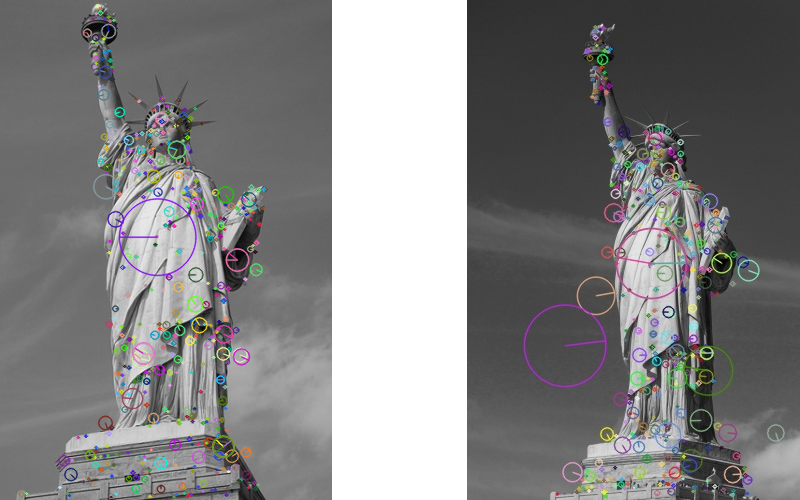
\includegraphics[scale=0.6]{images/liberty_kp.png}
	\caption{Gefundene \textit{keypoints} der beiden vorigen Bilder der Freiheitsstatuen farblich hervorgehoben (SIFT Detektor)}
	\label{img:keypoints}
\end{figure}

\subsection{Bildoperationen}

Zur Detektion und Extraktion von Features werden eine Reihe mathematischer Operationen und Verfahren genutzt, wie sie in der Bildverarbeitung üblich sind. Hiervon werden diejenigen vorgestellt, die im Weiteren der Arbeit verwendet werden.

\subsubsection{Histogramm}

Ein Histogramm ist eine diskrete Funktion, welche die Häufigkeitsverteilung in einer Menge abbildet. Hierfür wird jeder Wert der Menge einer Klasse zugeordnet. Die Größe der Intervalle einer Klasse leiten sich aus der Größe des gesamten Wertebereichs und der Anzahl der Klasse ab. So kann beispielsweise die Verteilung der Pixel eines Bildes auf die Intensitäten als Histogramm betrachtet werden. Bei einem monochromatischen Bild liegen 256 Intensitätswerte vor, die je eine Klassen repräsentieren. Beim Bilden des Histogramms wird jeder Pixels betrachtet und der Zähler der Klasse um eins inkrementiert, in deren Wertebereich der Intensitätswert des Pixels fällt. Ein Histogramm ist normalisiert, wenn es die relative Verteilung in der Menge darstellt.
In Abbildung \ref{img:hist} sind im Wesentlichen zwei Bereiche zu erkennen: ein sehr heller Hintergrund und eine dunkle Katze, die den Großteil des Bildes ausmacht. Dies spiegelt sich auch im Histogramm wieder: Es ist eine große Mengen an Punkten im dunklen Bereich vorhanden (Intensität $< 128$) und eine kleine, extreme Häufung im hellen Bereich.

\begin{figure}
	\centering
	\includegraphics[scale=0.8]{images/big_cat.png}
	\caption{Graustufenbild und Verteilung der Intensitätswerte}
	\label{img:hist}
\end{figure}

\subsubsection{Filter} 
Eine Filteroperation auf einem Bild soll bestimmte Bestandteile, z.B. Rauschen, reduzieren oder andere interessante Bereiche hervorheben. Dabei wird ein sogenannter Filterkern $F$, eine kleine Matrix von Koeffizienten, auf alle Teilbereiche des Bilders angewendet. 

\textbf{Gauß-Filter}
Ein Gauß-Filter wird in der Bildbearbeitung verwendet um ein Bild zu verzerren und somit Rauschen aber auch Details zu unterdrücken. Diesem Filter liegt, wie der Name sagt, die Gauß-Funktion zu Grunde:

$$
g_{\sigma}(x)=\frac{1}{\sqrt{2\pi\sigma^{2}}}\mathrm{e}^{-\frac{x^{2}}{2\sigma^{2}}}, \quad g_{\sigma}(x, y) = \frac{1}{\sqrt{2\pi\sigma^{2}}}\mathrm{e}^{-\frac{x^{2} + y^{2}}{2\sigma^{2}}}
$$

Wird ein Gauß-Filter verwendet, so bedeutet dies, dass die Einträge der Matrix aus der Gauß-Funktion konstruiert sind: $F_{G}(x, y) = g(x) * g(y)$. Da im Standardfall eine Nachbarschaft von $3 \times 3$ um den Pixel vorhanden sein muss, ergeben sich bei einem Bilder der Größe $n \times m$ Gradienten-Bilder der Größe $(n-2) \times (m-2)$.

\textbf{Difference of Gaussians}
Durch den Difference of Gaussian (DoG) Operator können insbesondere Kanten hervorgehoben werden. Wie der Name andeutet wird hier die Differenz zwischen zwei Bildern gebildet, auf die jeweils ein Gauß-Filter angewandt wurde. Hier variieren die Standardabweichungen der Gauß-Funktionen um zwei unterschiedlich stark verzerrte Versionen des Originals zu erzeugen. Hierbei gilt, dass die Standardabweichung $\sigma_{2} > \sigma_{1}$ ist:

$$ DoG(x, y, \sigma_{1}, \sigma_{2}) = I * G_{\sigma_2} - I * G_{\sigma_1}$$

\section{K-means Clustering}

Unter k-means Clustering werden Algorithmen zusammengefasst, die eine Menge Vektoren durch Zuweisung in $k$ vorgegebene Gruppen einteilen, die sogenannten Cluster. Aus den Vektoren werden initial $k$ Stück ausgewählt, die als anfängliche Schwerpunkte der Cluster dienen. Ein k-means Algorithmus ordnet nun iterativ jeden Vektor dem Cluster zu, der diesem am nächsten ist. Formal werden $n$ Vektoren aus dem Raum $\mathbb{R}^{d}$ in $k$ Cluster eingeteilt. $D$ ist hierbei eine Distanzmetrik im euklidischen Raum. Oft wird hier der quadrierte Fehler durch k-means minimiert, also beispielsweise $D = ||x_{i} - c_{j}||^{2}$. Jeder Vektor $x_{i}$ wird dem Cluster $c_{j}$ zugeordnet, dessen Distanz zum Vektor am Geringsten ist:

$$ X = \sum_{j=1}^{k} \sum_{i=1}^{n} min D(x_{i}, c_{j}) $$

Soll ein globales Optimum gefunden werden, so ist k-means NP-schwer. Praktische Implementierungen approximieren daher meist die Schwerpunkte der Cluster, wie beispielsweise der Algorithmus von Llyod. Zunächst beginnt Llyods Algorithmus mit einer Initialisierung der Schwerpunkte. Schritt zwei und drei werden dann solange wiederholt, bis der Algorithmus konvergiert, also die Vektor-Cluster-Zuordnung sich nicht mehr oder nur noch gering ändert oder eine maximale Anzahl an Iterationen erreicht wurde: 

\begin{enumerate}
	\item \textbf{Initialisierung} Es werden zunächst $k$ Vektoren durch ein Verfahren (z.B. zufällig oder \textit{farthest-neighbour}) als Schwerpunkte der Cluster ausgewählt.
	\item \textbf{Zuordnung}: Von den verbleibenden Vektoren wird nun mit jedem Cluster die neue Summe der Varianzen bei Aufnahme des Vektors berechnet. Es wird der Vektor dem Cluster zugeordnet, dessen Varianz sich am geringsten bei Aufnahme des Vektors erhöht.
	\item \textbf{Vektoren zuweisen}: Die Zentren der Cluster werden neu berechnet, um den neu zugeordneten Vektor in Folgeberechnungen miteinzubeziehen.
\end{enumerate}

Zur geometrischen Veranschaulichung sind in Abbildung \ref{img:kmeans} Punkte im zweidimensionalen Raum gegeben. Die Verteilung der Punkte ist in diesem Beispiel idealisiert, um bei einem Clustering mit einem $k = 3$, die Cluster in der rechten Grafik zu erhalten. Dies illustriert auch, dass abhängig von den Daten nicht immer sinvolle Cluster gebildet werden können. Die Wahl der initialen Clusterschwerpunkte kann das Ergebnis ebenfalls stark beeinflussen, daher sollte diese nicht immer zufäliig gewählt werden. \cite{mmd2011}

\begin{figure}
	\centering
	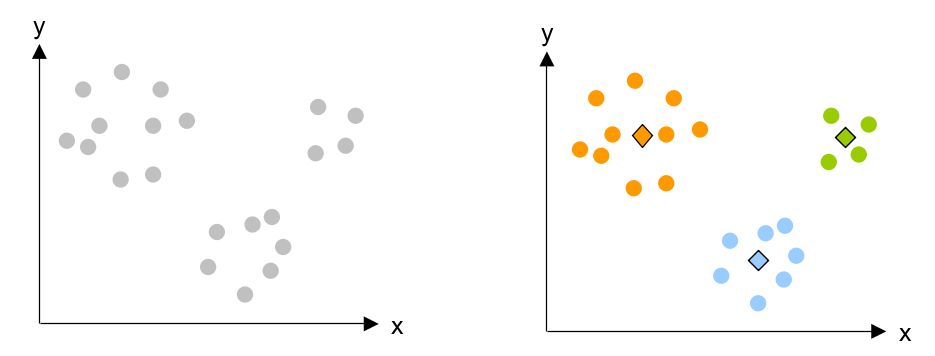
\includegraphics[scale=0.55]{images/kmeans.png}
	\caption{K-means Clustering im zweidimensionalen Raum mit $k = 3$.}
	\label{img:kmeans}
\end{figure}

\section{Neuronale Netze}

Neuronale Netze sind dem Aufbau und der Funktionsweise der Neuronen des menschlichen Gehirns nachempfunden. Es wird eine Menge von künstlichen Neuronen genutzt, um eine Lösung für ein Problem zu gestalten. Erste theoretische Überlegungen tauchten bereits in den 40er Jahren auf. Durch die wachsende Rechenleistung und neue Forschungsgebiete wie Machine Learning finden neuronale Netze seit Mitte der 80er Jahre vermehrt praktische Anwendung und akademische Zuwendung \cite{nnk2007}. Dadurch, dass neuronale Netze von Natur aus hoch parallel arbeiten können, eignen sie sich vor allem für parallele Architekturen und die Verarbeitung großer Datenmengen. 

\subsection{Modell}
Ein neuronales Netz besteht aus einer Menge Neuronen, die in Schichten im Netzwerk angeordnet sind. Jedes Neuron besitzt einen Aktivierungszustand und einen Schwellwert. Von diesen hängt ab, ob ein Signal weitergeleitet wird. Neuronen benachbarter Schichten sind vollständig durch gewichtete Kanten miteinander verbunden. Diese Beziehung wird in einer Gewichtsmatrix ausgedrückt. Eine Kante zwischen zwei Neuronen die nicht verbunden sind, hat dann den Wert 0 als Gewicht, um die Abwesenheit auszudrücken. 
Das Netz verarbeitet ein Signal, welches hier als Vektor $x \in [0,1]^n$ aus $\mathbb{R}^n$ dargestellt wird. Die erste Schicht des Netzwerks, der \textit{Input layer}, leitet das Signal nur an die nächste Schicht weiter und besitzt daher $n$ Neuronen. Die letzte Schicht, der \textit{Ouput layer}, dient zur Ausgabe des Ergebnisvektors $z \in [0,1]^m$, wobei $m$ die Anzahl der Elemente des Vektors angibt. Zwischen diesen beiden Schichten können sich beliebig viele \textit{Hidden layer} befinden. Die \textit{Hidden layer} bilden somit den Kern des Netzes, deren Kantengewichtungen, Kanten oder Neuronen während eines Lernprozess angepasst werden können. In Abbildung \ref{img:nnexample} ist ein Netz mit drei Schichten dargestellt. Der \textit{Input layer} nimmt einen Vektor mit vier Komponenten als Eingabe entgegen. Die Werte des Vektors werden an jedes der fünf Neuron im \textit{Hidden Layer} weitergeleitet, was durch die Kanten symbolisiert wird. Jede Kante besitzt dabei ein Gewicht, dass aus Gründen der Übersicht nicht aufgeführt ist. Schließlich werden die Ausgaben des \textit{Hidden layers} an das einzige Neuron des \textit{Output layers} geschickt und von diesem als Ergebnis $z$ ausgegeben.

\begin{figure}
	\centering

	\begin{tikzpicture}[shorten >=1pt,->,draw=black!50, node distance=\layersep]
    \tikzstyle{every pin edge}=[<-,shorten <=1pt]
    \tikzstyle{neuron}=[circle,fill=black!25,minimum size=17pt,inner sep=0pt]
    \tikzstyle{input neuron}=[neuron, fill=green!50];
    \tikzstyle{output neuron}=[neuron, fill=red!50];
    \tikzstyle{hidden neuron}=[neuron, fill=blue!50];
    \tikzstyle{annot} = [text width=6em, text centered]

    % Draw the input layer nodes
    \foreach \name / \y in {1,...,4}
        \node[input neuron, pin=left:$x_{\y}$] (I-\name) at (0,-\y) {};

    % Draw the hidden layer nodes
    \foreach \name / \y in {1,...,5}
        \path[yshift=0.5cm]
            node[hidden neuron] (H-\name) at (\layersep,-\y cm) {};

    % Draw the output layer node
    \node[output neuron,pin={[pin edge={->}]right:$z$}, right of=H-3] (O) {};

    % Connect every node in the input layer with every node in the
    % hidden layer.
    \foreach \source in {1,...,4}
        \foreach \dest in {1,...,5}
            \path (I-\source) edge (H-\dest);

    % Connect every node in the hidden layer with the output layer
    \foreach \source in {1,...,5}
        \path (H-\source) edge (O);

    % Annotate the layers
    \node[annot,above of=H-1, node distance=1cm] (hl) {Hidden layer};
    \node[annot,left of=hl] {Input layer};
    \node[annot,right of=hl] {Output layer};
	\end{tikzpicture}

	\caption{Beispiel eines dreischichtigen neuronalen Netzes.}
	\label{img:nnexample}
\end{figure}

Die Verarbeitung eines Signals in einem Neuron ist in Abbildung \ref{img:neuron} schematisch dargestellt und lässt sich in drei Schritte untergliedern:
\begin{itemize}
	\item \textbf{Propagierungsfunktion} Aus der Eingabe aller verbundenen Neuronen wird die Netzeingabe berechnet. Meist wird hier die gewichtete Summe zwischen Eingabe und Gewicht verwendet: $\sum_{i=1}^{} w_{i}x_{i} + b$. $b$ ist hier der sogenannter Bias-Vektor, der dazu verwendet werden kann Einfluss auf die Aktivierung zu nehmen.
	\item \textbf{Aktivierungsfunktion} Es wird der neue Aktivierungszustand des Neurons aus dem alten Zustand und der Netzeingabe durch die Aktivierungsfunktion $a$ berechnet. Häufig wird hier die ReLU (Rectified Linear Unit) $a_{ReLU}(x)=max(0,x)$ bzw. die Sigmoidfunktion $a_{s}(x) = 1/1+e^{-x}$ verwendet.
	\item \textbf{Ausgabefunktion} Wird ein Neuron aktiviert, so wird das resultierende Signal durch die Ausgabefunktion berechnet und an alle Neuronen in der folgenden Schicht weitergeleitet. Oft wird hier die Identitätsfunktion verwendet.
\end{itemize}

\begin{figure}
	\centering

	\begin{tikzpicture}[shorten >=1pt,->,draw=black!50, node distance=\layersepN]
    \tikzstyle{every pin edge}=[<-,shorten <=1pt]
    \tikzstyle{neuron}=[circle,fill=black!25,minimum size=27pt,inner sep=2pt]
    \tikzstyle{input neuron}=[neuron, fill=green!50];
    \tikzstyle{output neuron}=[neuron, fill=white!0];
    \tikzstyle{hidden neuron}=[draw, rectangle, minimum height=10mm, minimum width=10mm, fill=red!50];
    \tikzstyle{annot} = [text width=9em, text centered]

    % Draw the input layer nodes
    \node[input neuron, pin=left:$x_{1}$] (I-1) at (0,-1) {$w_{1}$};
	\node[input neuron, pin=left:$x_{2}$] (I-2) at (0,-2) {$w_{2}$};
    \node[input neuron, pin=left:$x_{n}$] (I-3) at (0,-3) {$w_{n}$};

    % Draw the sum
    \path[yshift=0.5cm]
    node[hidden neuron] (H-sum) at (\layersepN,-2.5cm) {$\sum$};

    % Draw the activation
    \path[yshift=0.5cm]
    node[hidden neuron] (H-act) at (\layersepN * 2,-2.5cm) {$s$};

    % Draw the output (invisible)
    \node[output neuron, right of=H-act] (O) {};

    % Connect input to sum
    \path (I-1) edge (H-sum);
    \path (I-2) edge (H-sum);
    \path (I-3) edge (H-sum);

	% Connect sum to act
    \path (H-sum) edge (H-act);

    % Connect act to output
    \path (H-act) edge (O);

    % Annotate the layers
    \node[annot,above of=H-sum, node distance=1.2cm] {Propagierungs-\\ funktion};
    \node[annot,above of=H-act, node distance=1.2cm] {Aktivierungs-\\ funktion};

	% Annotate edges
	\node[annot,above of=H-act, right=-0.3cm, node distance=0.2cm] {Aktivierung};
	\node[annot,above of=H-sum, right=-0.3cm, node distance=0.2cm] {Netzeingabe};
	
	\end{tikzpicture}

	\caption{Verarbeitung eines Signales in einem Neuron (ohne Ausgabefunktion).}
	\label{img:neuron}
\end{figure}

\subsection{Training eines Netzes}

Wurde ein neuronales Netz konstruiert, folgt darauf die Trainingsphase. Durch das Training ist es möglich, dass ein Netzwerk Neuronen oder Verbindungen hinzufügt bzw. entfernt, den Schwellwert für die Aktivierung von Neuronen verändert oder die Gewichte zwischen Neuronen anpasst. Pro Trainingselement wird die Fehlerquote $F$ zwischen dem angestrebten Ergebnis $z'$ und der Ausgabe des Netzes $z$ berechnet:
$$ F(z, z')=\sum_{i=0}^{n}(z'_{i} - z_{i})^2 $$
Durch eine Lernregel werden abhängig von der Fehlerquote beispielsweise die Gewichte der Kanten angepasst. Für Netze ohne \textit{Hidden layer} eignet sich hier die Hebbsche oder Delta Lernregel. Für Netze mit mindestens einem \textit{Hidden layer}, hat sich das \textit{Backpropagation} Verfahren etabliert. \textit{Backpropagation} minimiert den Gradientenabstieg auf der Fehleroberfläche die $F$ aufspannt. Der Algorithmus geht in drei Schritten vor:

\begin{enumerate}
	\item \textbf{Forward Pass} Die Gewichte des Netzwerks werden initialisiert und eine Eingabe durch das Netz propagiert. Als Resultat liegt die Ausgabe vor.
	\item \textbf{Fehlerberechnung} Die Fehler des \textit{Output layers} werden, durch einen Vergleich mit den erwarteten Werten, berechnet. Falls die Fehler unterhalb einer vorgegebenen Grenze liegen, ist das Training beendet. Andernfalls wird fortgefahren.
	\item \textbf{Backward Pass} In diesem Schritt wird die Fehlerquote rückwärts durch das Netz propagiert. Die Gewichte an den Verbindungen zwischen Neuronen werden in Abhängigkeit ihres Einflusses auf den Fehler Schicht für Schicht aktualisiert.
\end{enumerate}

\section{CUDA}

Der Begriff CUDA ist ein Akronym für \textit{Compute Unified Device Architecture}. Dahinter verbirgt sich eine Architektur von Nvidia für parallele Berechnungen durch Grafikkarten. Das Umsetzen von Programmen auf Grafikkarten, die nicht mit der Verarbeitung von grafischen Daten in Zusammenhang stehen, wird GPU Computing (Graphics Processing Unit Computing) genannt. Die meisten GPU Computing Ansätze, und auch CUDA, verwenden als Ausführungsmodell das Single Program Multiple Data (SPMD) Modell. Im Unterschied zum Multiple Instruction Multiple Data (MIMD) Modell, dass in CPUs verwendet wird, wenden alle Prozessoren das gleiche Programm auf unterschiedliche Daten an. Durch diese Art der Parallelisierung konnten in den letzten Jahren enorme Steigerungen der Gleitkommaoperationen pro Sekunde (flops) und der Speicherbandbreite bei Berechnungen erzielt werden. 
Hier wird im wesentlichen ein Einblick in die im CUDA C Programming Guide \cite{cud2012} detailliert beschriebenen Dokumentation gegeben, sodass ein Leser Teile eines CUDA Programms nachvollziehen kann. Zunächst wird näher auf das Ausführungsmodell und dessen Umsetzung eingegangen. CUDA unterscheidet zwischen verschiedenen Speicherbereichen auf der Grafikkarte. Da die Verwendung der unterschiedlichen Speicherbereiche wesentliche Unterschiede in der Implementierung eines Algorithmus und dessen Laufzeit zur Folge hat, werden diese im Kapitel \ref{cudaMemory} Speicherverwaltung behandelt. Um den praktische Einsatz von CUDA zu illustrieren, wird abschließend ein Programm zur Addition zweier Vektoren auf der Grafikkarte.

\subsection{Ausführungsmodell}

Ein Programm, dass auf einer Nvidia Grafikkarte ausgeführt werden soll, muss in der Sprache CUDA C geschrieben sein. Aus der Sicht eines Programmierers handelt es sich hierbei um eine Erweiterung von C um Primitive und Funktionen für Berechnungen auf der Grafikkarte. Zum Übersetzen und Linken des Codes dient der \textit{nvcc} Compiler von Nvidia. Dieser unterscheidet zwischen Code der auf dem \textit{host}, der CPU, und dem \textit{device}, der GPU, ausgeführt wird. Das Kompilieren von \textit{host} Code erfolgt durch den auf dem \textit{host} installierten C Compiler. Der \textit{device} Code wird durch \textit{nvcc} zu PTX bzw. cubin binary code übersetzt.
Nvidia hat das SPMD Modell durch \textit{kernels} umgesetzt. Ein \textit{kernel} ist ein Programm, dass parallel auf verschiedene Daten der GPU angewendet wird. 
Bevor ein \textit{kernel} aufgerufen werden kann, muss der notwendige Speicher auf der Grafikkarte für die Daten und das Ergebnis allokiert werden. Anschließend werden die Daten von \textit{host} zu \textit{device} kopiert. Nach Durchführung der Berechnung kann dann das Ergebnis zurück zum \textit{host} kopiert werden. Die Datentransfers weisen eine nicht unbeachtliche Latenz auf. Folglich sollte das Kopieren von Daten nur selten erfolgen.
Die Daten liegen in der Regel als Vektor oder Matrix vor. Der Zugriff auf verschiedene Elemente durch unterschiedliche \textit{kernel} erfolgt dann durch eine Indexberechnung. Diese wird anhand des Beispiels der Vektoraddition näher erläutert.
Beim Aufruf des \textit{kernels} muss die Anzahl der Threads pro Block und die Anzahl der Blocks in einem Grid angegeben werden. Ein Block ist eine logische Einheit und entspricht einem Multiprozessor der Grafikkarte. Durch diese Strukturierung können die Blöcke parallel auf der Hardware ausgeführt werden. Das Grid enthält die Blöcke und kann ein, zwei oder dreidimensional sein. In Abbildung \ref{img:cuda1} ist ein eindimensionales Grid mit sechs eindimensionalen Blöcken á 12 Threads schematisch dargestellt. Ein Block kann auf aktuellen Grafikkarten bis zu 1024 Threads beinhalten.

\begin{figure}
	\centering
	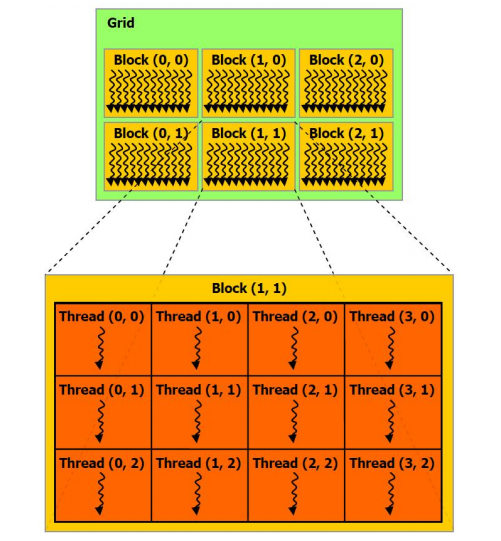
\includegraphics[scale=0.55]{images/cuda1.png}
	\caption{Organisierung von Threads in Blocks in Grids \cite{cud2012}}
	\label{img:cuda1}
\end{figure}

\subsection{Speicherverwaltung}
\label{cudaMemory}

Dadurch, dass die Daten vom \textit{host} zum \textit{device} kopiert werden müssen und vice versa, unterscheidet cuda zwischen \textit{host memory} und \textit{device memory}. Darüber hinaus ist der \textit{device memory} bereits auf der Grafikkarte in verschiedene Bereiche organisiert, wie in Abbildung \ref{img:cuda_mem} dargestellt. Jeder Multiprozessor hat Zugriff auf den \textit{global memory} sowie einen eigenen lokalen \textit{shared memory}, \textit{Constant} und \textit{Texture Cache}. Lokal erstellten Variablen werden als \textit{Register} bezeichnet. Auf diese ist der Zugriff mitunter am schnellsten, jedoch sind sie lokal pro Thread. Die Daten liegen als Parameter zunächst im \textit{global memory} vor. Im \textit{Constant Cache} liegen alle durch das cuda Schlüsselwort \textit{\textunderscore\textunderscore constant\textunderscore\textunderscore} deklarierte Werte. Zugriffe auf den \textit{global memory} sind am langsamsten, da der Speicherbereich zwischen allen Multiprozessoren geteilt wird und Zugriffe mitunter synchronisiert werden müssen \todo{HARDWARE}. Durch Verwendung des \textit{shared memory} und \textit{texture cache} können Speicherzugriffe beschleunigt werden, jedoch können Daten aus diesen Bereichen nicht zwischen Blöcken geteilt werden.

\begin{figure}
	\centering
	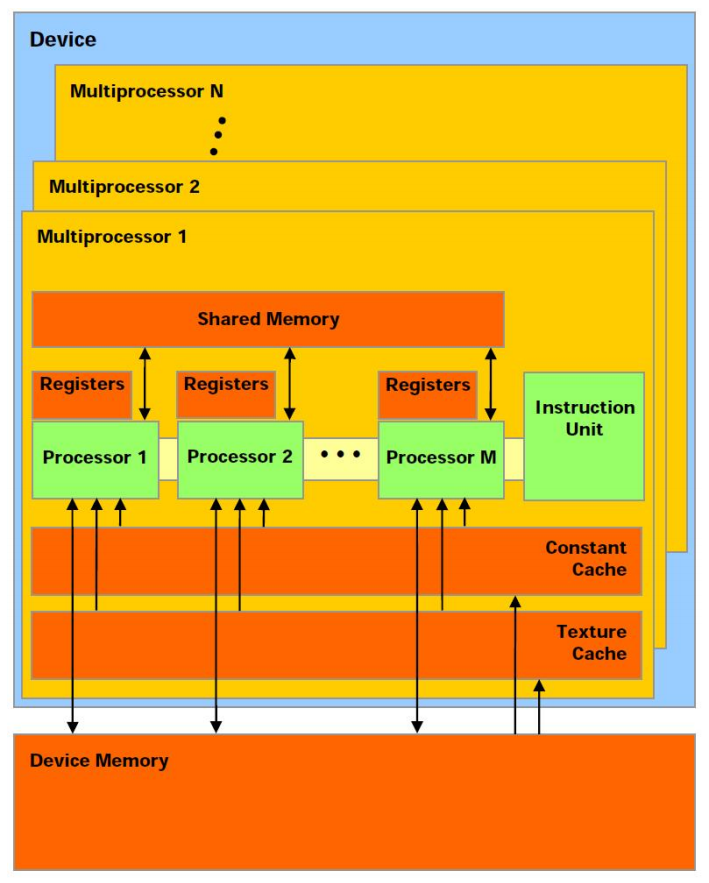
\includegraphics[scale=0.4]{images/cuda_mem.png}
	\caption{Organisierung der verschiedenen Speichertypen}
	\label{img:cuda_mem}
\end{figure}

\subsubsection{Shared Memory}

Gerade bei vielen parallelen Lese- / Schreibzugriffen kann hier eine hohe Latenz auftreten, wenn viele Threads auf die gleichen Adressen zugreifen. Aus diesem Grund empfiehlt es sich, die benötigten Daten von dem \textit{global} in den \textit{shared memory} zu kopieren. Der \textit{shared memory} wird von allen Threads in einem Block geteilt. Beim Kopieren der Daten muss ein Index berechnet werden, um die korrekten Daten dem jeweiligen Block zuzuordnen. Soll beispielsweise jeder \textit{kernel} auf dem Element eines Vektors arbeiten, setzt sich der globale Index aus der Position im Block und im Thread zusammen: $blockDim.x * blockId.x + threadId.x$. Die Variablen $blockDim$ und $blockId$ sind, wie $threadId$, durch CUDA gesetzt. Weiterhin ist zu beachten, dass nicht beliebig viel \textit{shared memory} allokiert werden kann: Je nach Grafikkarten stehen pro Block zwischen 16 und 48 Kilobyte Speicher zur Verfügung. 
Durch den Einsatz von \textit{shared memory} können gegenüber Algorithmen die exklusiv den \textit{global memory} nutzen, wesentliche Steigerung in der Performance (hier: kürze Laufzeit) erreicht werden. Allerdings ist der \textit{shared memory} mit 16 bzw. 48 Kilobyte sehr begrenzt und erhöht die Komplexität durch notwendiges Kopieren von Daten und Indexberechnungen.

\subsection{Vektoraddition}

Am Beispiel der Vektoraddition soll der Aufbau und Ablauf eines cuda Programms illustriert werden. Hierfür wird zunächst die Funktion \textit{vecAdd} angelegt. Hier wird in Zeile 8 - 10 durch \textit{cudaMalloc} der benötigte Speicher für die Vektoren und das Ergebnis allokiert. Anschließend werden die Daten von Vektor $a$ und $b$ zum \textit{device} kopiert. In den beiden folgenden Zeilen wird der Inhalt der Vektoren $a$ und $b$ vom \textit{host} zum \textit{device} kopiert. In Zeile 15 wird der \textit{kernel} \textit{add} aufgerufen, der auf der Grafikkarte ausgeführt wird. Einem \textit{kernel} muss durch Angabe in den dreifachen spitzen Klammern, die Dimension des Grids und der Blocks mitgeteilt werden. Im Beispiel werden pro Block 256 Threads verwendet (\textit{numThreads}) und die Anzahl der notwendigen Blocks aus der Vektorgröße und der Threadanzahl berechnet. Da die Verarbeitung asynchron erfolgt, wird durch \textit{cudaDeviceSynchronize} in der nächsten Zeile die Ausführung auf dem \textit{host} pausiert, bis die GPU fertig ist. In Zeile 17 wird das Ergebnis vom \textit{device} zurück zum \textit{host} kopiert und kann ausgegeben oder weiterverarbeitet werden.
Der \textit{kernel} wird von jedem Thread ausgeführt. Jeder Thread kümmert sich um die Addition eines Elementes aus $a$ und aus $b$ am selben Index. Damit dieser Index global eindeutig ist, muss neben der $threadId$ in x-Richtung die Grid und Blockdimension des Threads berücksichtigt werden. Falls der berechnete Index innerhalb der Vektoren liegt, wird die Summe in $c$ geschrieben.

\lstset{language=C}
\begin{lstlisting}
void vecAdd (float *a, float *b, float *c, int size) {
	int numThreads = 256;
	int numBlocks = (size + numThreads - 1) / numThreads;
	float *aPtr = 0;
	float *bPtr = 0;
	float *cPtr = 0;	
	
	cudaMalloc((void **) aPtr, a, sizeof(float) * size);
	cudaMalloc((void **) bPtr, b, sizeof(float) * size);
	cudaMalloc((void **) cPtr, c, sizeof(float) * size);	
	cudaMemcpy(aPtr, a, sizeof(float) * size, cudaMemcpyHostToDevice);
	cudaMemcpy(bPtr, b, sizeof(float) * size, cudaMemcpyHostToDevice);	
	
	add<<<numBlocks, numThreads>>>(aPtr, bPtr, cPtr, size);
	cudaDeviceSynchronize();
	
	cudaMemcpy(c, cPtr, mem, cudaMemcpyDeviceToHost);
	
	cudaFree(aPtr);
	cudaFree(bPtr);
	cudaFree(cPtr);
}

__global__ void add (float *a, float *b, float *c, int size) {
	int id = blockDim.x * blockIdx.x + threadIdx.x;
	if (id < size) c[id] = a[id] + b[id];
}
\end{lstlisting} 

